\subsubsection{导航技术总览}
\noindent\textbf{用语说明：}视觉组四个方向之一是\textbf{导航}，赛场上主要落地在哨兵等移动平台。本章的激光雷达（LiDAR）是测距传感器，与方向名“雷达站”不是一回事。

现在，你坐在哨兵的脑袋里面，你的目标是悄悄摸到敌方基地后面偷家。
但是没认真看规则的你忘记了地图长什么样，你打开手机，发现好心的wzx部长已经帮你存了一份\textbf{标准赛场地图[1]}。
于是你打开\textbf{缺德地图[2]}，把赛场地图传上去。你又打开手机GPS，把自己的\textbf{定位[3]}也告诉缺德地图，
最后，你输入目的地，缺德地图就帮你规划好了一条用时最少的路。
于是你就跟着这条路径走，同时你并没有关掉GPS，这样才知道自己有没有走错。
在路上，你在\textbf{视野[4]}里看到了许多其他机器人，你以你秋名山车神的\textbf{车技[5]}，在他们之间穿梭，避开了所有车。
突然！What can I say, man!无人机坠机坠在了你前进的道路上。
你对车身大小了如指掌。只看一眼，你计算出哨兵过不去，路被堵了。
鉴于无人机死状惨烈，这无人机短时间是飞不起来，你走不了这条路了。
不过还好，每隔一段时间，缺德地图会再算一次路径，你可能会听到“正在为您重新规划路径”，他帮你找到了另一条路。
虽然“缺德地图持续为您服务”，但是有时候你可能会开到一些“信号不好”，无法获取缺德地图服务的地方。
此时，你要能够在不依靠缺德地图的情况下\textbf{自己找到[6]}信号比较好能重新连接上缺德地图服务的地方。
最终你成功到达了目的地。


\begin{figure}[H]
\centering
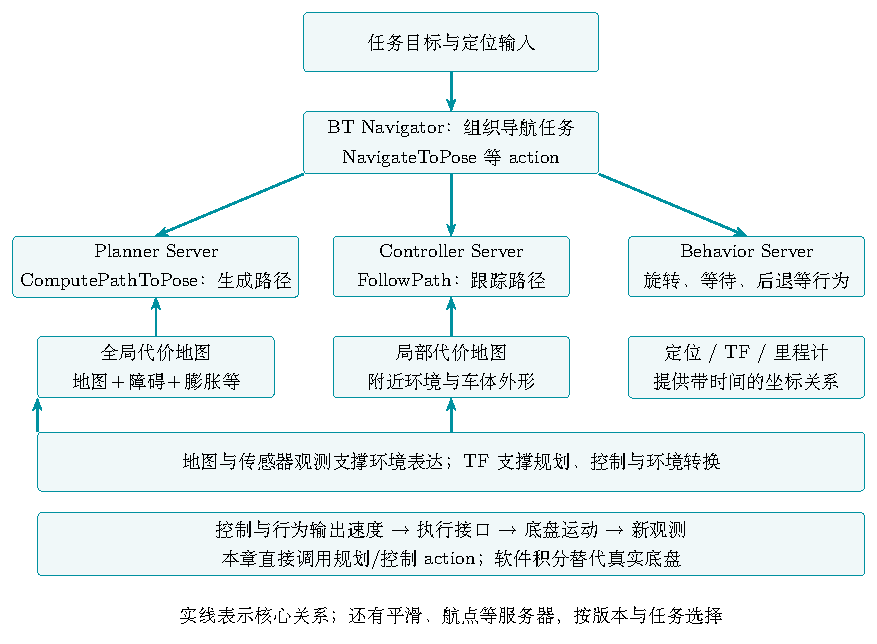
\includegraphics[width=.94\textwidth]{nav_framework_revised.pdf}
\caption{Nav2 的核心调用与数据关系；并非所有项目都只启动这几个服务器}
\label{fig:I_nav-1}
\end{figure}

先别急着给哨兵装手机，我们把刚才的六样东西对上号。[1]是记录场地的\textbf{地图（Map）}，它还要经过障碍更新、外形与通行余量等处理，才成为全局代价地图（Global Costmap）。[2]相当于整个导航系统，其中负责找路的是\textbf{规划器（Planner）}。[3]是\textbf{定位（Localization）}，其结果通过带时间的位姿、TF 等接口传给其他模块；TF 是坐标关系，自己不会凭空算出位置。[4]对应不断更新的\textbf{局部代价地图（Local Costmap）}。[5]对应\textbf{控制器（Controller）}，根据路径、位姿和附近障碍算出速度。[6]则是\textbf{恢复（Recovery）}策略，由任务逻辑决定什么时候等、什么时候重试，以及什么时候向上层报告失败。

不过，手机“信号不好”只是帮助记忆的类比。真实机器人可能是 TF 缺失、观测过期、没有可行控制或长期不前进，处理方式各不相同，不能一律先倒车再说。我们先定位，给规划器当前位置和目标；规划器给出路径，控制器跟踪，新的障碍进入代价地图后还可能触发重规划。这几个模块一直交换最新数据，才形成导航闭环。

\begin{example}\label{ex:nav-overview}
这章的小项目在本卷的 \texttt{examples/navigation/navigation-lab-demo}。首先在 Ubuntu 22.04 的 Humble 环境安装依赖，再进入项目。下面的路径是仓库位置示例，换成你自己的；使用 Distrobox 时，先进入已安装 Humble 的 Ubuntu 22.04 容器；示例容器名换成你自己的，原生 Ubuntu 用户跳过这一步。
\begin{tbash}
distrobox enter ubuntu2204
bash
source /opt/ros/humble/setup.bash
sudo apt-get install --no-install-recommends \
  ros-humble-navigation2 ros-humble-nav2-bringup \
  libpcl-dev cmake g++ python3-numpy python3-scipy \
  python3-matplotlib python3-yaml fonts-wqy-zenhei
cd /home/mijiao/Apps/Tutorial4New/02-专项技术栈/\
examples/navigation/navigation-lab-demo
export ROS_DOMAIN_ID=188
export ROS_LOCALHOST_ONLY=1
\end{tbash}
本章代码与配置使用 Humble 的 Nav2 接口，PCL 由系统的 libpcl-dev 提供。两终端需要同一套环境与 Domain ID；188 是演示选择，若本机已有项目使用它就换一个空闲值。

我们用生成的小地图，让真实 Nav2 服务器规划、控制，再由软件积分速度，观察机器人是否真的沿路前进。地图、TF、最短路和恢复的代码会在相应小节依次展开，完整调用在\ref{sec:nav-real}节。
\end{example}
\begin{exercise}\label{ex:nav-chain}
已有路径却没有速度输出，先查哪一段？如果连当前位置都拿不到，为什么反复点“重新规划”通常没用？画出你要检查的两个数据链。
\end{exercise}

\subsubsection{先把坐标关系接起来}
我们上一章让云台转到了某个角度，导航现在要回答“小哨兵在场地哪里”。在 ROS 中，变换（Transform）描述两个坐标系（Frame）的相对平移和旋转；一组有父子关系的变换就组成 TF 树。车体、雷达、相机都有自己的坐标系，查询一条连通路径，才能把某个雷达点换算到地图里。

\begin{figure}[H]
\centering
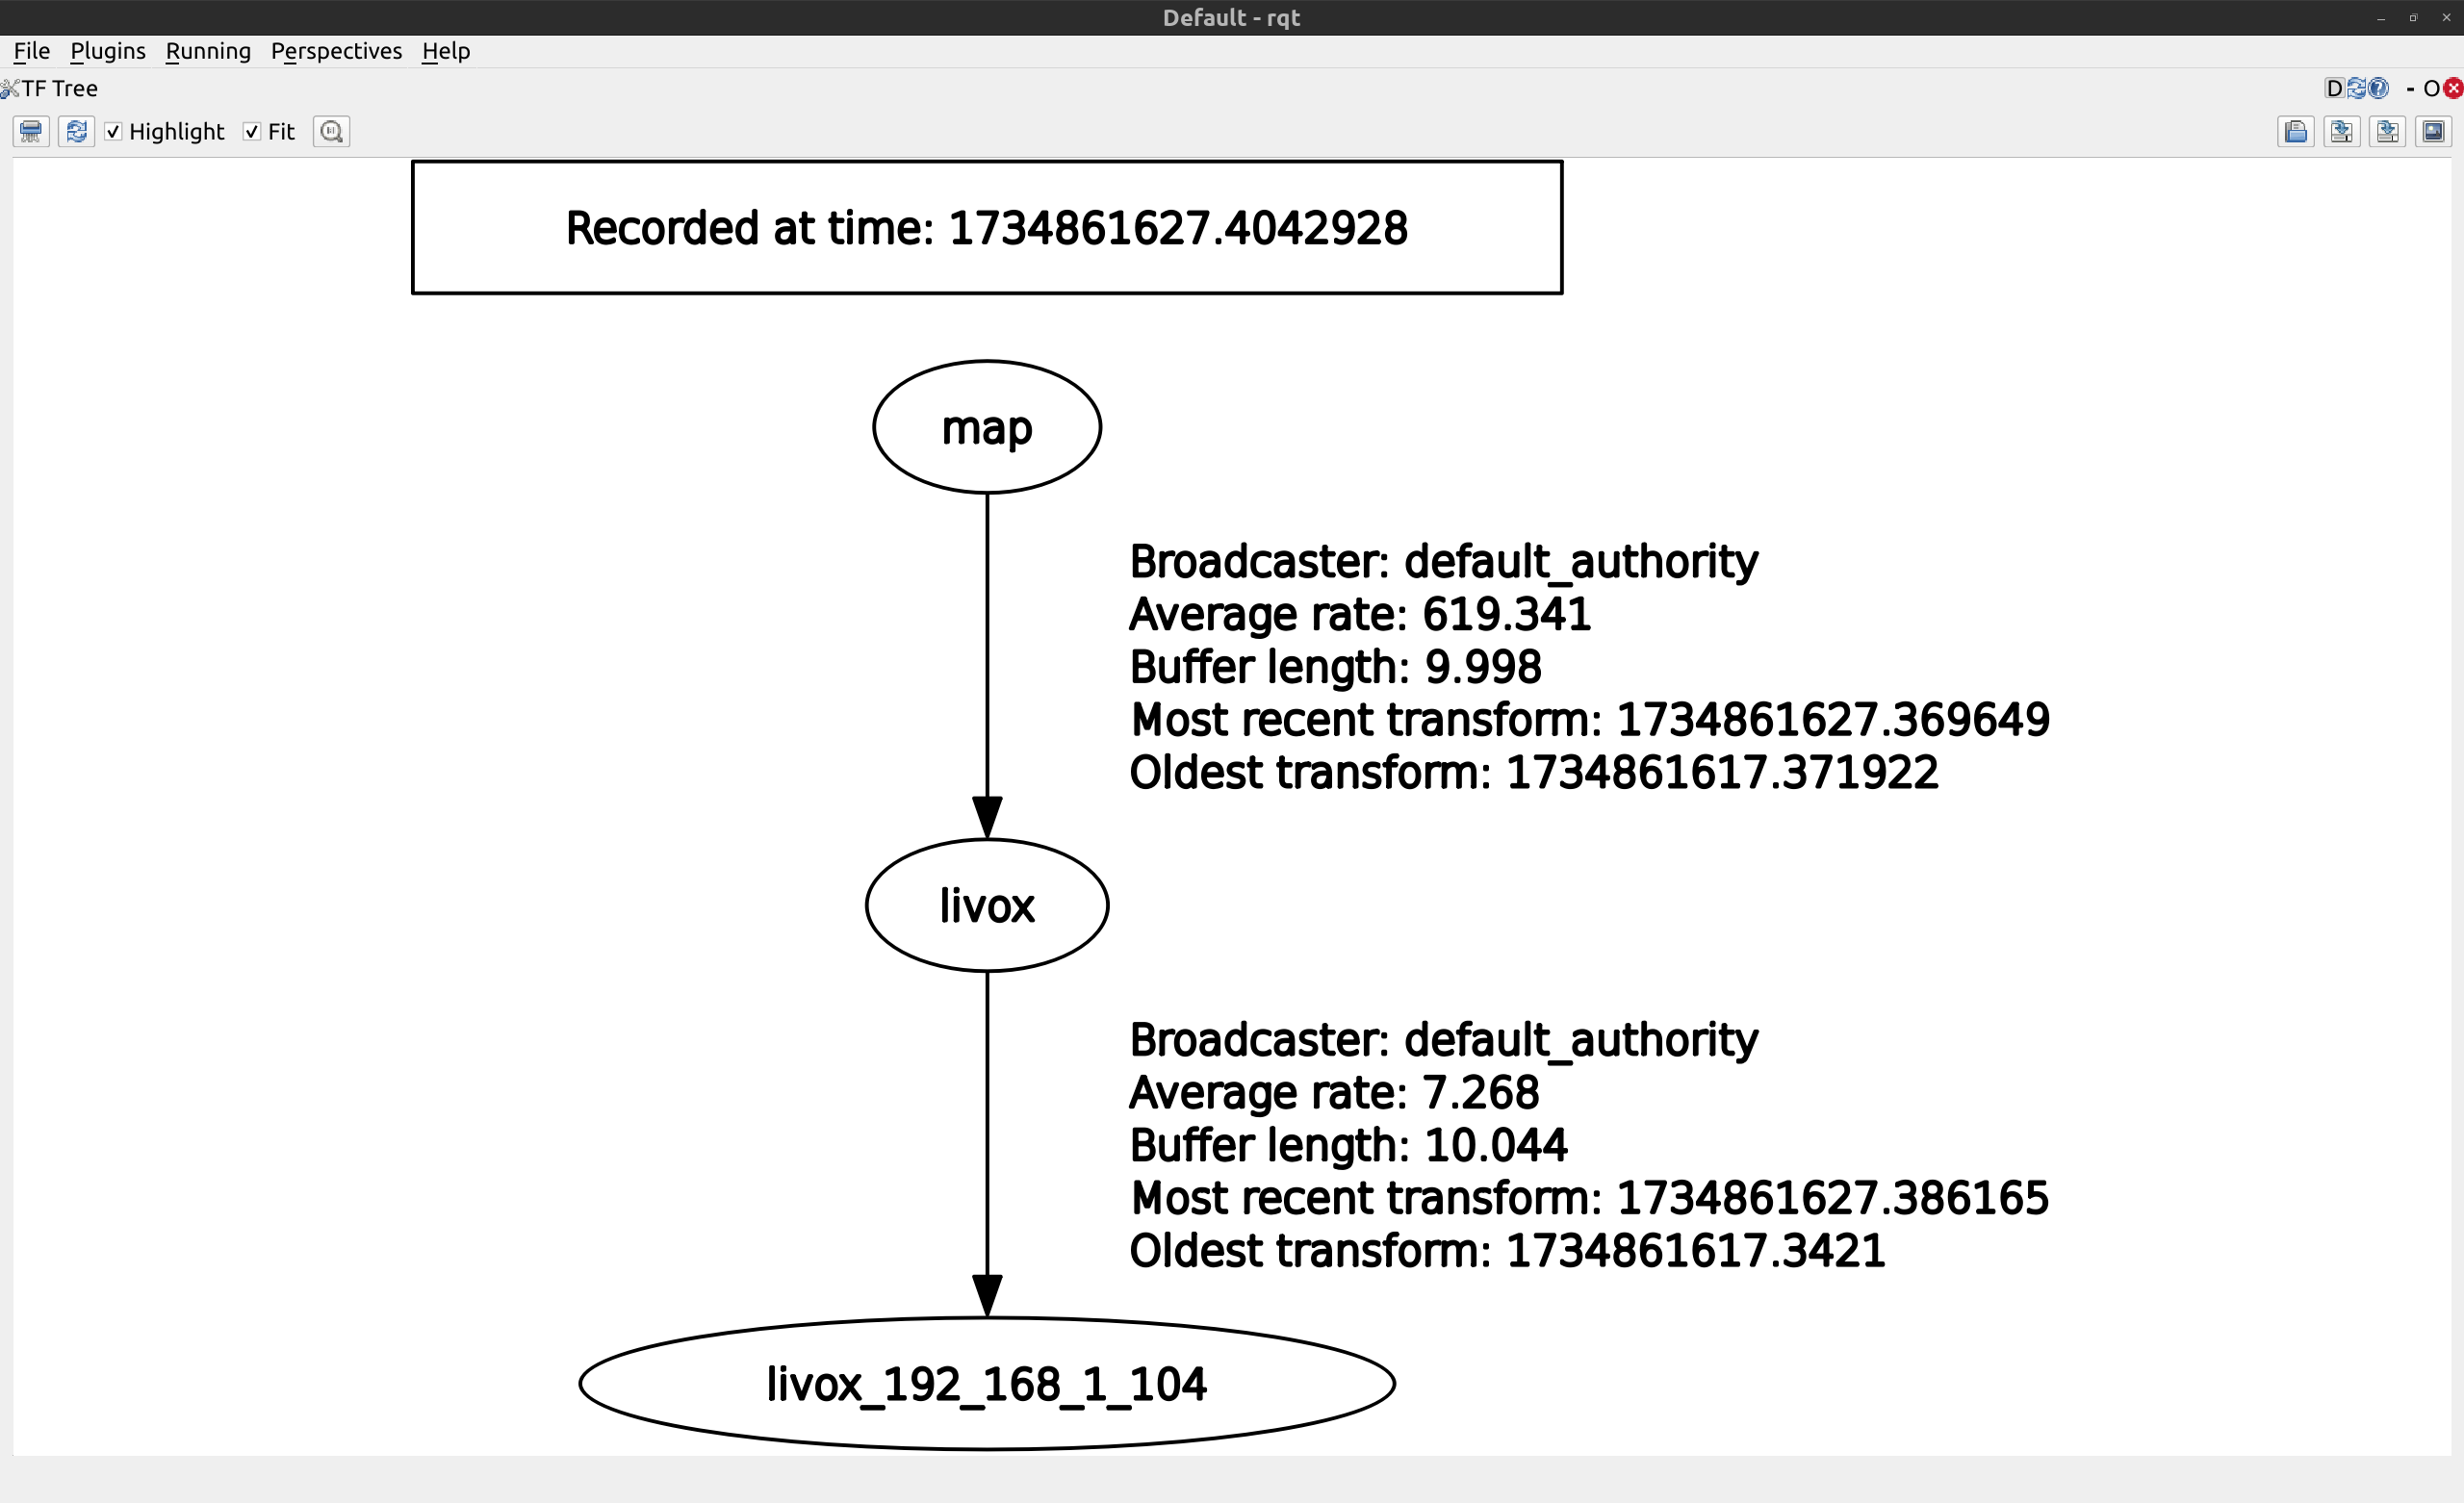
\includegraphics[width=.8\textwidth]{tf树_revised.png}
\caption{原项目的真实 TF 截图，记录 map、livox 与设备坐标系；图中的时间和频率保留原值，不能当成本章实验结果}
\label{fig:I_nav-2}
\end{figure}

名字通常用 \texttt{map}、\texttt{odom}、\texttt{base\_link}、\texttt{camera\_link}、\texttt{laser\_link}。它们是坐标系名称，开头不要加话题名那样的斜杠。图\ref{fig:I_nav-2}是原项目自定义关系的例子；想接入常见的移动机器人导航链，我们更常采用图\ref{fig:I_nav-3}的约定。
\begin{figure}[H]
\centering
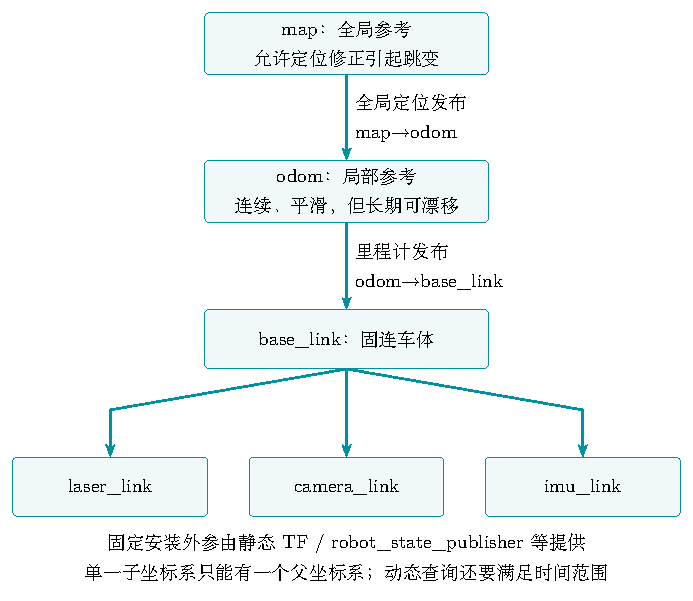
\includegraphics[width=.89\textwidth]{nav_frames_revised.pdf}
\caption{REP-105 的常见地图、里程计和车体关系；每个子坐标系只有一个父坐标系}
\label{fig:I_nav-3}
\end{figure}

\texttt{odom} 要让短时间的位置变化平滑、连续，即使走久了会漂；\texttt{map} 要对齐全局场地，定位修正时允许跳变；\texttt{base\_link} 固连车体。通常里程计发布 \texttt{odom→base\_link}，全局定位发布 \texttt{map→odom}，安装外参发布车体到传感器的固定变换。不要让两个节点抢着发布同一个子坐标系，不然哨兵可能没动，坐标先吵起来了。各坐标系的职责可对照\href{https://github.com/ros-infrastructure/rep/blob/master/rep-0105.rst}{REP-105 原文}。

\begin{example}
先做一条最简单的静态变换。终端一保持运行，终端二查询：
\begin{tbash}
# 终端一；只用独立演示坐标系
ros2 run tf2_ros static_transform_publisher \
  --x 1 --y 0 --z 0 --yaw 0 --pitch 0 --roll 0 \
  --frame-id demo_map --child-frame-id demo_base
# 终端二
ros2 run tf2_ros tf2_echo demo_map demo_base
\end{tbash}
稍等发现完成，应看到平移 $(1,0,0)$ 和零旋转。停止终端一后把 x 改为 2，再启动同一个发布程序，核对新的平移。不要同时启动两份发布者。
\end{example}

\begin{example}
一条边会查了，我们再查询两条边合成后的结果。\texttt{tf\_demo.py} 使用真实 tf2 Buffer 存入独立静态变换：第一条平移 $(1,2)$、旋转 $90^\circ$；第二条在父坐标系里沿 x 平移 2。代码完整如下：
\lstinputlisting[language=Python,basicstyle=\footnotesize\ttfamily]{examples/navigation/navigation-lab-demo/tf_demo.py}
\begin{tbash}
python3 tf_demo.py
\end{tbash}
输出约为 \texttt{xy: [1,4]}，缺失分支是 \texttt{LookupException}。为什么不是 $(3,2)$？因为第二条的 x 轴已经转向了地图的 y 轴。TF 连通还不够，动态变换也要覆盖查询时间；查旧时刻或未来时刻时出现外推异常，要先检查时间戳、时钟和缓存，不能靠把所有变换设为静态解决。
\end{example}
\begin{exercise}\label{ex:nav-tf}
完成 x=1 与 x=2 的命令实验，然后把 \texttt{tf\_demo.py} 第一条旋转改为零，预测并核对合成结果。解释真实 map→odom 为何不能长期用一个固定值代替。
\end{exercise}
\begin{conclusion}
地图负责全局一致，里程计负责局部连续，车体负责固定参考。位置可用要同时满足树连通、时间可查、单位与方向正确。TF 是这些关系的传递工具，定位算法才负责估计它们。
\end{conclusion}

\subsubsection{定位、建图和融合到底在忙什么}
导航里常听到 \textbf{SLAM（Simultaneous Localization and Mapping，同时定位与建图）}，简称 SM（不是）。定位可以在已有地图上匹配当前位置；SLAM 则在未知环境中同时估计自己的运动和地图，所以“所有定位都必须先有地图”并不成立。

可怜的小哨兵在场馆里通常没有可直接使用的 GPS，只好看周围的墙、柱子，读车轮和 IMU。激光雷达发射光并接收返回信号，测距后结合扫描角度得到点，有的还提供回波强度。将当前扫描与已有地图或局部子地图对齐，再结合雷达到车体的外参，就能估计车体位置。三维方法如 ICP、NDT，二维方法如基于栅格地图的 AMCL，各有适用条件；三维保留了高度信息，不意味着任何场景都一定更准确，精度和耗时还取决于几何、噪声、初值与实现。

局部匹配通常只看附近或最近的地图，让运动估计及时更新；全局重定位则扩大搜索范围，处理刚上电不知道在哪、位置已经明显不对等情况。不过，重定位不是“清空 TF，再把车体位置归零”。我们要用新的全局估计修正 map→odom，让 odom→base\_link 继续平滑，控制器才不会突然把定位修正当成底盘瞬移。

\begin{example}
设里程计认为车体在 $(2,0.5)$，地图匹配认为它在 $(2.3,0.5)$。按照变换相乘关系，
\[
T_{map,base}=T_{map,odom}T_{odom,base},\qquad
T_{map,odom}=T_{map,base}T_{odom,base}^{-1}.
\]
我们用 \texttt{localization.py} 跑一下这个修正，也顺便看看长走廊为什么容易让雷达迷路。
\lstinputlisting[language=Python,basicstyle=\footnotesize\ttfamily]{examples/navigation/navigation-lab-demo/localization.py}
\begin{tbash}
python3 localization.py
\end{tbash}
第一次 map→odom 的平移是 $(0.3,0)$；全局估计改为 $(2.2,0.5)$ 后修正变成 $(0.2,0)$，而里程计坐标仍是 $(2,0.5)$。两面沿 x 无限延伸的墙只约束横向，代码里的法向量矩阵特征值是 0 和 2，沿 x 移动 100 m 仍产生零墙面残差。这是几何退化的极简演示：实际走廊如果能看到端点、柱子等特征，纵向仍可能受到约束，不能把这两个数当成真实雷达定位误差。
\end{example}
\begin{exercise}\label{ex:nav-localization}
地图估计改成 $(1.8,0.7)$，计算新的 map→odom 平移。再给墙面约束增加法向量 $(1,0)$，运行查看新的特征值，说明它补上了哪个方向的信息。
\end{exercise}

轮式里程计把车轮运动累加起来，打滑会积累误差；IMU（Inertial Measurement Unit，惯性测量单元）测角速度和比力，要处理重力、偏置、安装方向与积分漂移，不能把读出的加速度直接加到地图坐标上。视觉里程计（Visual Odometry，VO）利用图像特征或像素变化估计运动，单目尺度、光照、遮挡、纹理都可能影响结果，也没有一个“视觉精度一定比激光低”的通用排名。

所以我们让传感器互相补位：轮子短时间走得连贯，地图匹配给全局修正，IMU 提供较快的运动信息。但“融合”也不是把三个坐标平均一下，外参、时间同步、噪声和退化条件都要先说清楚。否则融合的可能只是三份不同步的错误。第八章的滤波和第九章的几何优化，就是你继续深入时会用到的工具。

\begin{figure}[H]
\centering
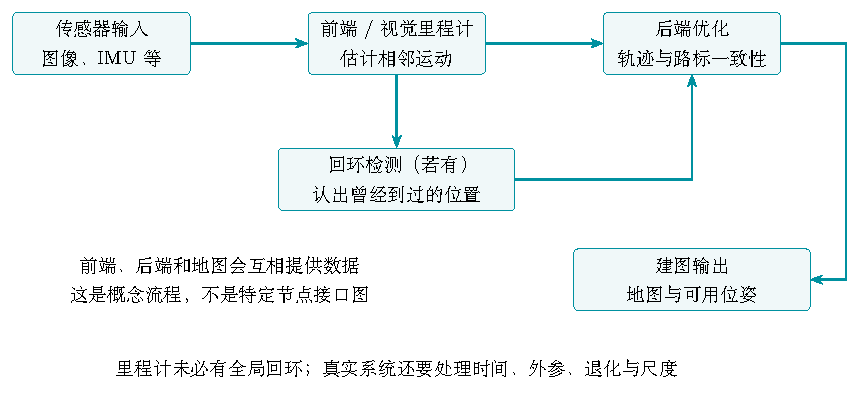
\includegraphics[width=.92\textwidth]{nav_slam_revised.pdf}
\caption{常见视觉 SLAM 的概念流程；回环可以修正累计误差，但不是所有里程计系统都有回环模块}
\label{fig:I_nav-4}
\end{figure}

从求解方式看，可以看到滤波与图优化两类思路，但具体系统经常组合使用。gmapping 使用粒子滤波；hector\_mapping 的核心是扫描匹配，不能一起塞进“都是滤波”的筐里。\href{https://index.ros.org/p/hector_mapping/}{hector\_mapping 的介绍}可以帮助核对这一点。Point-LIO 是激光惯性里程计的例子，\href{https://github.com/hku-mars/Point-LIO}{其原仓库}强调点时间戳、雷达与 IMU 同步、外参和 IMU 量程；原版提供的是 ROS 1 构建流程，接 ROS2 Humble 时还要核对实际采用的移植版本。这里没有把它装上就宣布“小哨兵会定位了”，本章先把输入输出和故障原因对上。
\begin{exercise}\label{ex:nav-fusion}
一份雷达数据落后 IMU 0.1 s，车体以 1 m/s 平移。仅考虑这个时间差，两份数据对应的位置会相差多少？再分别给出轮子打滑、白墙缺纹理和长走廊中的一个排查方向。
\end{exercise}
\begin{conclusion}
已有地图上的定位、连续运动估计和同时建图承担不同任务。回环是再次认出到过的地方并施加一致性约束，既可能纠正轨迹，也可能纠正地图；它不是凭空把所有误差清零。先问清传感器提供什么、哪个方向可观测，再选择融合或优化方法。
\end{conclusion}

\subsubsection{先把点云收拾一下}
导航需要地图。小哨兵还没学会飞行，我们先用二维导航表达，但 z、roll、pitch 仍会影响坡道、车体高度和传感器投影。地图通常可以从三维点云处理得到，也可以直接使用二维扫描建图。激光测到的主要是可见表面，没看到的地方不能自动当成空地。

首先，近处点云太密，全部计算容易变成“三帧电竞”，这时候可以用\textbf{体素下采样（Voxel Grid）}。PCL 的 VoxelGrid 把同一体素内的点合成\textbf{质心}，不是固定的体素几何中心。叶子尺寸越大，点越少，细小障碍也更可能被抹掉；不要只盯着帧率。

然后，用\textbf{直通滤波（Pass Through）}留下某个坐标范围。z 范围要先统一到合适坐标系，再根据车体可碰撞高度选择。雷达装在车顶时，“z 大于 0.5”未必就是离地 0.5 m；横梁、桌面等也可能让车体过不去，不能因为点在某个高度之外就宣判安全。

\textbf{统计离群点移除（Statistical Outlier Removal，SOR）}则计算点到 K 个近邻的平均距离，以全局均值加标准差倍数作阈值。这是对邻域平均距离分布的假设，不是“所有点坐标都符合高斯分布”。稀疏的真实障碍也可能被误删，所以换场地、换密度时要看滤前滤后。

\begin{example}
\texttt{point\_filters.cpp} 自己生成两组小点云，不需要雷达。第一组只有两个点，让你看清质心；第二组放入 30 个近点、1 个远离群点和 1 个低点，分别观察直通与 SOR。
\lstinputlisting[language=C++,basicstyle=\footnotesize\ttfamily]{examples/navigation/navigation-lab-demo/point_filters.cpp}
完整构建配置是 \texttt{CMakeLists.txt}，这里同时启用 C 与 C++，兼容 PCL 依赖中可能出现的 C/MPI 目标。
\lstinputlisting[language=bash,basicstyle=\footnotesize\ttfamily]{examples/navigation/navigation-lab-demo/CMakeLists.txt}
\begin{tbash}
cmake -S . -B build
cmake --build build -j4
./build/point_filters
\end{tbash}
实测输出为质心 x=0.02、输入 32、直通后 31、统计过滤后 30。0.1 m 体素的中心 x 是 0.05，这就能直接区分“体素中心”和“点的质心”。PCL 的\href{https://pointclouds.org/documentation/tutorials/voxel_grid.html}{VoxelGrid 教程}与\href{https://pointclouds.org/documentation/tutorials/statistical_outlier.html}{SOR 教程}可查参数；网页版本可能更新，本例在 PCL 1.14.0 上实际编译运行。
\end{example}
\begin{exercise}\label{ex:nav-filter}
将两个点的 x 改为 0.01 和 0.09，先手算质心，再同步修改程序中的核对值并运行。若叶子尺寸改为 0.02，它们还在同一个体素吗？说明为什么不能为了让程序返回 0 就忽略真实输出。
\end{exercise}

最后还有地面提取。简单的 z 截取、平面拟合、法向量和聚类都能提供线索，但“最大聚类就是地板”“平的就是地板”都只是特定场景的假设。桌面也平，墙面也可能是最大一组点，我们还要结合高度、朝向、连续性与场地结构。原项目的法向量方法可以保留为工程选择，阈值与误删风险应通过真实地面和障碍样本验证，这部分放到卷三建图实验。

\subsubsection{把地图保存完整，再谈哪里能走}
现在，你拿到了某个时刻附近的点。要拼成完整地图，先用每一帧的位姿把它们变到共同坐标系，再处理动态物体、遮挡和误差，不能把传感器原坐标下的数组直接叠起来。三维地图常存为 PCD；二维栅格通常由 PGM/PNG 图片与 YAML 元数据共同表示。尽量保留无损图片，JPG 的压缩边缘可能影响障碍判定。

栅格索引 $(i,j)$ 对应的不是格角而是格心。设分辨率 r、地图原点 $(o_x,o_y)$ 和偏航 $\psi$，先得到局部格心，再旋转平移：
\[
\begin{bmatrix}x\\y\end{bmatrix}=
\begin{bmatrix}o_x\\o_y\end{bmatrix}+
\begin{bmatrix}\cos\psi&-\sin\psi\\\sin\psi&\cos\psi\end{bmatrix}
\begin{bmatrix}(i+0.5)r\\(j+0.5)r\end{bmatrix}.
\]
所以宽 W、高 H 格的地图覆盖 $Wr\times Hr$，只把图片缩放一下而不改元数据，场地就会被你偷偷放大或缩小。图像通常从顶部开始数行，而地图从较小 y 向上数；没有旋转时，第 v 行对应 $j=H-1-v$。

\begin{example}\label{ex:nav-grid-project}
我们把栅格换算、生成输入和找路放进同一个 \texttt{grid.py}。本小节先看 \texttt{cell\_center} 和生成 PGM/YAML 的部分；\texttt{shortest} 与 \texttt{plan} 在下一小节继续使用，所以这里给出完整文件，后面直接对照。
\lstinputlisting[language=Python,basicstyle=\footnotesize\ttfamily,firstline=1,lastline=43]{examples/navigation/navigation-lab-demo/grid.py}
\lstinputlisting[language=Python,basicstyle=\footnotesize\ttfamily,firstnumber=44,firstline=44]{examples/navigation/navigation-lab-demo/grid.py}
\begin{tbash}
python3 grid.py --output out/map
python3 -c 'from grid import cell_center; print(\
cell_center(10,20,.05,(0,0,0)))'
cat out/map/map.yaml
\end{tbash}
第二行得到 $(0.525,1.025)$ m。生成图固定 60×40 格、0.1 m/cell，也就是 6×4 m，黑色边框和中央矩形是人为障碍。保存时上下翻转，\texttt{map.yaml} 的内容如下，图片路径相对 YAML 所在目录解释：
\begin{tbash}
image: map.pgm
mode: trinary
resolution: 0.1
origin: [0.0, 0.0, 0.0]
negate: 0
occupied_thresh: 0.65
free_thresh: 0.25
\end{tbash}
这是三值地图模式：图像灰度经 negate 规则转换为占据概率，再按两个阈值分类。ROS 的占据栅格（OccupancyGrid）用 -1 表示未知、0～100 表示占据；Nav2 原始代价地图有另一套 0～255 的编码。未知不等于自由，两套数组也不能不转换就直接交换。
\end{example}
\begin{exercise}\label{ex:nav-map}
把原点改为 $(-2,-1)$，求同一个 $(10,20)$ 格心。如果改为原点 $(1,2)$、偏航 $90^\circ$、分辨率 0.1，求 $(2,3)$ 格心并用函数核对。40 行图片的第 0 行对应哪个地图 j？
\end{exercise}
\begin{note}
定位地图应保留可复核的几何信息。禁止通行区用导航约束表达，编辑前保留原始版本，再核对实际场地；把未知刷成白色只是骗过规划器，墙不会因为你修图就消失。
\end{note}

\subsubsection{给路径算代价，也给车留空间}
地图能帮助定位，但要找路，还需要代价地图（Costmap）：自由区域代价低，越靠近障碍代价越高，致命障碍不能通过。为了方便“掺点小料”，Nav2 用地图层（Layer）插件组合信息。静态层（Static Layer）接收已有地图，障碍层（Obstacle Layer）根据观测标记、清除障碍，体素层（Voxel Layer）可保留高度信息，膨胀层（Inflation Layer）在障碍周围生成代价分布，通常放在要膨胀的障碍层之后。

哨兵不是不计体积的理想质点，膨胀层因此堂堂登场。不过，调一个 inflation\_radius 就不代表完成了碰撞检查，还要正确配置车体轮廓（Footprint）或半径，并留出定位、离散化和控制误差的余量。KeepoutFilter 和 SpeedFilter 是代价地图过滤器，配置接口与普通 layer 有区别，分别表达禁止区和区域限速；区域限速不能替代底盘本身的速度上限。

全局代价地图供较大范围的规划，局部代价地图供附近控制；内容和更新速度由任务决定，不是固定的“三层对两层”。本项目已知一张静态地图，所以两张代价地图都使用静态层与膨胀层；没有伪装成雷达正实时扫描动态障碍。

\begin{example}
假设车速 v=2 m/s、可用制动减速度 a=1 m/s$^2$，理想制动距离为 $v^2/(2a)=2$ m；再加 0.2 s 的总延迟，至少多走 0.4 m。若机器人位于 4 m 方形局部窗口的正中心，正前方可见长度只有 2 m，这还没算余量就不够。窗口应覆盖预测、停车与观测需求，频率也要能在预算内完成，不是越快越好。

离线 \texttt{plan} 用障碍格心距离大于 margin 判断可通行，\texttt{--margin} 默认 0.35 m。它只是四邻接算法实验的模型，不是完整 Nav2 footprint 检查。运行 \texttt{python3 grid.py --margin 0.6 --output out/wide}，比较通道变窄后的路线；margin 大到起终点也被挡住时，代码明确返回无路。
\end{example}
\begin{exercise}\label{ex:nav-costmap}
速度保持 2 m/s、延迟仍为 0.2 s，将减速度改为 2 m/s$^2$，计算不含额外余量的前向距离需求。5 m 方形窗口的半宽够不够？再解释清空动态障碍层为什么不应清掉静态墙。
\end{exercise}
\begin{conclusion}
图片是地图输入，地图层组合成代价地图，外形检查与控制再决定运动是否可行。全局地图不能自动看到新障碍，局部地图也不能只靠扩大范围补救过期观测。配置外形、更新范围、延时和制动能力时，要把它们放在同一个量级里看。
\end{conclusion}

\subsubsection{现在终于可以找路了}
有了地图和定位，我们进入正题。Dijkstra 在非负边权图上，每次取累计代价最小的候选点向外扩展；普通广度优先搜索只有在各边等权时才能直接这样求最低代价。A* 则按 $f(n)=g(n)+h(n)$ 选候选点，其中 g 是已经走过的代价，h 是到目标的估计。

本例的四邻接就是每格只连接上下左右四格。在 \texttt{grid.py} 的四邻接图里每步代价为 1，曼哈顿距离不高估剩余步数，并满足一致性，所以 A* 可以更有方向地找到同样最低代价的路线。若随手把 h 乘十，或者用了与边权不匹配的距离，就不能继续宣称最优。最少拐弯、最短距离、最快时间，也不是同一个优化目标；Nav2 插件的结果由代价与约束共同决定。
\begin{example}
先跑三顶点图，再对照上面的完整 \texttt{shortest}：
\begin{tpython}
from grid import shortest
graph = {"A": [("B", 1), ("C", 5)],
         "B": [("C", 2)], "C": []}
print(shortest(graph.__getitem__, "A", "C"))
\end{tpython}
输出路径 A→B→C、代价 3。返回值还记录取出的候选点次数，用于比较这份实现的搜索工作量。再运行：
\begin{tbash}
python3 grid.py --output out/map
python3 grid.py --blocked --output out/blocked
\end{tbash}
默认地图中两算法总代价均为 70、路径均有 71 格；本实现 Dijkstra 扩展 1304 次，A* 扩展 914 次，数量也受相同代价时的取点顺序影响。\texttt{--blocked} 加入一面贯穿地图的墙，二者都返回空路径和 \texttt{cost: null}。返回“无路”才是合理结果，不能为了完成任务穿墙。
\end{example}
\begin{exercise}\label{ex:nav-search}
将三顶点图 A→C 改为 2，运行核对；再看默认栅格，解释为什么 A* 与 Dijkstra 同代价却可能取到不同路线。若边权为负，程序怎样处理？
\end{exercise}

\subsubsection{让规划出的路径真的变成运动}\label{sec:nav-real}
如果只有规划器会怎么样？想象你在游戏里给角色指定了远处目标：
\begin{figure}[H]
\centering
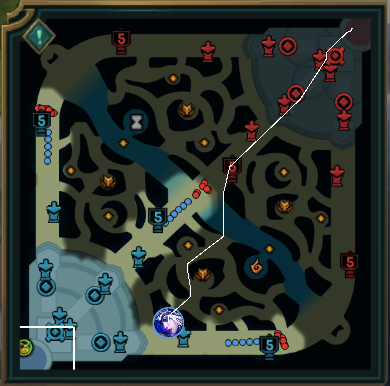
\includegraphics[width=.48\textwidth]{英雄联盟_revised.png}
\caption{原游戏小地图，用来类比全局路线；截图本身不能证明游戏使用了 A*}
\label{fig:I_nav-5}
\end{figure}
规划时没看到的移动目标可能突然挡路，只有路线还不够。回到缺德地图，你这位车手对应控制器，地图只告诉你怎么绕到目的地，你还要根据视野和车的能力决定眼下怎样转向、减速。Nav2 控制器通常输出 Twist 或 TwistStamped 速度，而不是直接替底盘算电机电流；电控执行接口还要在卷三接起来。

DWA、TEB 是常见的局部规划思路，但不能看到 Nav2 就默认它们正在运行。本章在 Humble 中明确选 Navfn 规划器和调节纯追踪（Regulated Pure Pursuit，RPP）控制器。RPP 根据前方追踪点与几何关系跟踪路径，同时调节速度并检查碰撞；它不是任意动态障碍下都能自行绕路的控制器。算法与参数可对照\href{https://github.com/ros-navigation/navigation2/tree/humble/nav2_regulated_pure_pursuit_controller}{Humble 的 RPP 说明}，实际插件以加载日志与配置为准。

\begin{example}\label{ex:nav-real-run}
首先看 \texttt{params.yaml}。\texttt{GridBased}、\texttt{FollowPath} 是我们给插件实例起的名字，后面的 action 请求要用相同 ID。控制频率 20 Hz；局部窗口 4×4 m；车体用半径 0.15 m 的圆；膨胀半径 0.35 m。配置使用 Humble 的 Twist 输出，没有速度平滑器、真实传感器或碰撞监控器。
\lstinputlisting[language=bash,basicstyle=\footnotesize\ttfamily,firstline=1,lastline=36]{examples/navigation/navigation-lab-demo/params.yaml}
接下来是两张代价地图的完整配置：
\lstinputlisting[language=bash,basicstyle=\footnotesize\ttfamily,firstnumber=37,firstline=37]{examples/navigation/navigation-lab-demo/params.yaml}

然后，\texttt{sim.py} 接收实际 \texttt{cmd\_vel}，用单调时钟的实际间隔积分平面运动，发布 odom 和 TF。固定 map→odom 为单位变换，是因为软件模型没有定位漂移；它明确替代了本实验的定位输入，不能搬到真实哨兵上当定位系统。
\lstinputlisting[language=Python,basicstyle=\footnotesize\ttfamily]{examples/navigation/navigation-lab-demo/sim.py}
该模型忽略惯性、打滑和碰撞动力学，断流 0.5 s 后只让软件停止积分。导航避障取决于实际代价地图和控制器检查，最后还应检查保存轨迹是否与障碍相交。

\texttt{lab.launch.py} 把 map\_server、planner\_server、controller\_server、生命周期管理器和软件模型一起启动。生命周期管理器负责配置、激活服务器，\texttt{map} 启动参数替换地图文件位置；整个示例不需要新建 ROS 包。
\lstinputlisting[language=Python,basicstyle=\footnotesize\ttfamily]{examples/navigation/navigation-lab-demo/lab.launch.py}

最后，\texttt{client.py} 等服务器真正激活，再调用 \texttt{ComputePathToPose}，成功后才调用 \texttt{FollowPath}。它订阅并保存真实服务器输出的速度和软件 odom，超时会请求取消，失败则保留 action 状态。Humble 的这两个 action 结果没有 \texttt{error\_code} 字段；成功与否用状态判断，具体失败原因从启动终端日志定位。进度检查器由服务器的 \texttt{progress\_checker\_plugin} 指定，不在 FollowPath 请求中另设 ID。
\lstinputlisting[language=Python,basicstyle=\footnotesize\ttfamily,firstline=1,lastline=50]{examples/navigation/navigation-lab-demo/client.py}
\lstinputlisting[language=Python,basicstyle=\footnotesize\ttfamily,firstnumber=52,firstline=52]{examples/navigation/navigation-lab-demo/client.py}
两个终端都进入项目、加载同一 ROS 环境和隔离 Domain，然后运行：
\begin{tbash}
# 终端一：先生成地图，launch终端保持运行
python3 grid.py --output out/map
ros2 launch "$PWD/lab.launch.py"
# 终端二
python3 client.py --output out/nav2
ros2 topic type /cmd_vel
ros2 param get planner_server GridBased.plugin
ros2 param get controller_server FollowPath.plugin
ros2 run tf2_ros tf2_echo map base_link
\end{tbash}
看到 \texttt{Managed nodes are active} 后地图与服务器已经激活；刚启动时短暂的“等待 TF”与一直超时不是同一种情况。客户端也会检查生命周期，避免“action 能连上，地图却还没准备好”的竞争。

正常完成时，规划状态和跟踪状态应均为 4（Succeeded），最终位置误差应在配置的 0.1 m 容差附近；路径点数以当前规划结果为准。具体 odom/速度样本数随运行调度变化，以你保存的 \texttt{result.json} 为准。本例应能观测到 60×40 的 map 和 global costmap；map 的值是 0/100，原始 costmap 中还有 253、254 和一系列膨胀代价，能看出它们不是同一数组。
\end{example}
\begin{exercise}\label{ex:nav-run}
实际启动该闭环，保存结果，核对插件 ID、cmd\_vel 类型、路径长度和最终位置误差。然后运行 \texttt{python3 client.py --blocked-goal --output out/nav2-blocked}，目标落在障碍中；它有没有继续调用控制器？从日志指出中断位置。
\end{exercise}

\begin{example}
现在把保存的数据画出来。\texttt{plot.py} 只读上面那次结果，不另造一条“看上去很成功”的轨迹。
\lstinputlisting[language=Python,basicstyle=\footnotesize\ttfamily]{examples/navigation/navigation-lab-demo/plot.py}
\begin{tbash}
python3 plot.py --map out/map --nav2 out/nav2 \
  --output out/navigation.pdf
\end{tbash}
默认字体使用依赖里的文泉驿，\texttt{--font} 可换成你机器上的中文字库；教材插图使用 Fandol 与其他章协调。左图看离线格心路线，右图看真实 Navfn 路径与软件轨迹，两边的模型与代价不同，不要求路径点一一重合。
\begin{figure}[H]
\centering
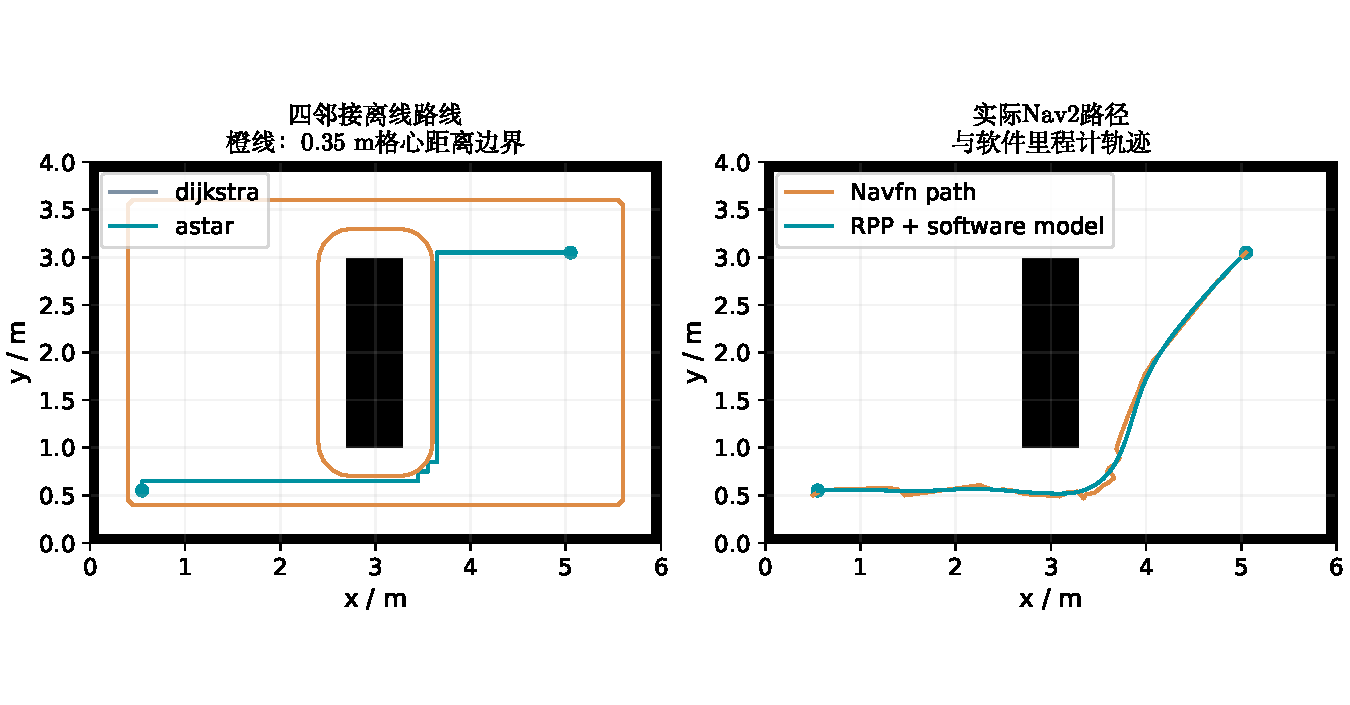
\includegraphics[width=.96\textwidth]{nav_paths_revised.pdf}
\caption{一组保存数据：四邻接离线路线与 Nav2 的规划、跟踪结果}
\label{fig:nav-paths}
\end{figure}
\end{example}
\begin{exercise}\label{ex:nav-plot}
把 \texttt{desired\_linear\_vel} 改为 0.3，停止终端一并重新启动，从同一初始位置跑到同一目标，保存到另一个输出目录。比较实际速度峰值与到达时长；说明为什么不能只改图上的标签就声称已经验证了慢速运行。
\end{exercise}
\begin{note}
项目输出目录用于保存当前实验，重复运行同一路径会覆盖数据。终端一 Ctrl+C 结束本项目；演示没有连接真实底盘，不应把这些配置直接启动在正在运动的机器人环境里。本章的圆形模型与静态场地软件验证，不能证明真实底盘制动、雷达覆盖或动态避障能力。
\end{note}

\subsubsection{失败以后，别让哨兵无限重试}
规划无路、控制无有效速度、进度长期不变时，任务需要选择恢复。清空过时障碍信息、等障碍离开、重新规划、旋转或后退都有用途，但要针对原因：清地图不能清掉真实墙，倒车也要先核对后方可行空间；TF 丢失时更应该修复数据链，而不是盲目转圈。

Nav2 的行为树（Behavior Tree，BT）用任务节点和控制节点组织流程。执行节点调用规划、控制或行为服务器；顺序（Sequence）按顺序执行，失败就停；选择（Fallback）只在当前分支失败时才试下一分支。节点返回 Success、Failure 或 Running；Running 表示还没完成，必须向上传递，不能一边跟踪路径一边误启动恢复。具体还有带记忆、响应式等控制节点，名称相似也要看执行语义。

\begin{example}
\texttt{bt.py} 是可以逐 tick 运行的等价教学模拟器，\texttt{Control} 实现带记忆的顺序/选择节点，\texttt{Recovery} 在导航失败后轮流清理、等待，成功才重试导航，最多完成两次恢复；恢复分支自己失败则立即退出。这与实际 Nav2 的\href{https://docs.nav2.org/rolling/configuration_and_development/configuration_guide/core_servers/bt_plugins/controls/RecoveryNode/}{RecoveryNode 重试职责}相对应，但本文件不是 Nav2 插件，也没有真的删代价地图。
\lstinputlisting[language=Python,basicstyle=\footnotesize\ttfamily,firstline=1,lastline=35]{examples/navigation/navigation-lab-demo/bt.py}
\lstinputlisting[language=Python,basicstyle=\footnotesize\ttfamily,firstnumber=36,firstline=36]{examples/navigation/navigation-lab-demo/bt.py}
\begin{tbash}
python3 bt.py
python3 bt.py --fail
python3 bt.py --stuck
\end{tbash}
默认日志依次为导航失败、清理成功、导航失败、等待 Running、等待成功、导航成功，最终重试计数为 2。\texttt{--fail} 让导航持续失败，恢复两次后结束为 Failure；\texttt{--stuck} 让等待一直 Running，十次 tick 后外层预算输出 Timeout。这个 tick 预算不是秒级实时保证，真实任务还要结合时钟期限和取消逻辑。

要直接核对 Fallback 的 Running 传播，可以在项目目录执行：
\begin{tpython}
from bt import Control, Script, RUNNING, SUCCESS
log = []
root = Control([Script("follow", [RUNNING], log),
                Script("recover", [SUCCESS], log)], sequence=False)
print(root.tick(), log)
\end{tpython}
只应记录 \texttt{follow}，不会调用 \texttt{recover}。真实导航的完整 BT XML 应结合已安装版本查看，BT Navigator 组织的不止规划与控制，还可以调用行为、平滑等服务，不能把导航软件永久写成“一大三小”。
\end{example}
\begin{exercise}\label{ex:nav-bt}
用 \texttt{Control} 分别核对两个分支均 Failure 的 Fallback、第一分支 Running 的 Sequence。再运行三种恢复序列，记录每次 tick 的返回值，解释恢复次数和 tick 预算各自限制什么。
\end{exercise}
\begin{conclusion}
规划器说“路在哪”，控制器说“现在怎么动”，恢复逻辑说“失败后怎么办”。恢复次数要有限，Running 要有上层时间预算，最终失败要能通知任务决策；让哨兵原地重试到比赛结束，日志可能挺努力，任务还是没完成。
\end{conclusion}
